\documentclass[12pt,a4paper,oneside]{article}
\usepackage[utf8]{inputenc}
\usepackage[czech]{babel}
\usepackage[T1]{fontenc}
\usepackage{float}
\usepackage{graphicx}
\usepackage{index}
\usepackage{url}
\author{Roman Ondráček}
\title{Dálkové ovládání domácích spotřebičů mobilním telefonem}
% Vytvoření seznamu použitých zkratek
\newindex{zkr}{zdx}{znd}{Seznam použitých zkratek}
\begin{document}
% Řádkování 1,5
\renewcommand{\baselinestretch}{1.5}
% Vynechání číslování
\pagestyle{empty}
% Zvětšení oblasti tisku pro tuto stránku
\enlargethispage{60mm}
\begin{center}
\large \textbf{STŘEDOŠKOLSKÁ ODBORNÁ ČINNOST} \\

\vspace{32mm}
% Český název
\huge \textbf{Dálkové ovládání domácích spotřebičů mobilním telefonem} \\

\vspace{64mm}
\end{center}

\begin{tabbing}
% Nastavení zarážek
\hspace{4mm} \= \hspace{24mm}  \=   \kill
\> \large \textbf{Autor:}  \> \large{Roman Ondráček}                                    \\[4mm]
\> \large \textbf{Škola:}  \> \large{Gymnázium Boskovice, příspěvková organizace}       \\[4mm]
\> \large \textbf{Kraj:}   \> \large{Jihomoravský}                                      \\[4mm]
\> \large \textbf{Obor:}   \> \large{10. Elektrotechnika, elektronika a telekomunikace} \\[24mm]
\> \large \textbf{Boskovice 2017}
\end{tabbing}

\newpage

% Řádkování 1,5
\renewcommand{\baselinestretch}{1.5}
% Vynechání číslování
\pagestyle{empty}
% Zvětšení oblasti tisku pro tuto stránku
\enlargethispage{60mm}
\begin{center}
\large \textbf{STŘEDOŠKOLSKÁ ODBORNÁ ČINNOST} \\

\vspace{32mm}
% Český název
\huge \textbf{Dálkové ovládání domácích spotřebičů mobilním telefonem} \\
\vspace{16mm}
% Anglický název
\huge \textbf{The remote control of home appliances via a mobile phone} \\

\vspace{24mm}
\end{center}

\begin{tabbing}
% Nastavení zarážek
\hspace{4mm} \= \hspace{24mm}  \=   \kill
\> \large \textbf{Autor:}     \> \large{Roman Ondráček}                                    \\[4mm]
\> \large \textbf{Škola:}     \> \large{Gymnázium Boskovice, příspěvková organizace}       \\[4mm]
\> \large \textbf{Kraj:}      \> \large{Jihomoravský}                                      \\[4mm]
\> \large \textbf{Školitel:}  \> \large{prof. Ing. Václav Říčný, CSc.}                     \\[4mm]
\> \large \textbf{Obor:}      \> \large{10. Elektrotechnika, elektronika a telekomunikace} \\[16mm]
\> \large \textbf{Boskovice 2017}
\end{tabbing}

\normalsize

\newpage

~ \vspace{88mm}

\section*{Prohlášení}

Prohlašuji, že svou práci na téma Dálkové ovládání domácích spotřebičů mobilním telefonem jsem vypracoval samostatně pod vedením prof. Ing. Václava Říčného, CSc. a s použitím odborné literatury a dalších informačních zdrojů, které jsou všechny citovány v práci a uvedeny v seznamu literatury na konci práce. \\
Dále prohlašuji, že tištěná i elektronická verze práce SOČ jsou shodné a nemám závažný důvod proti zpřístupňování této práce v souladu se zákonem č.~121/2000 Sb., o právu autorském, o právech souvisejících s právem autorským a změně některých zákonů (autorský zákon) v platném změní. \\[8mm]
V Boskovicích dne \today \hspace{24mm} Podpis: 

\newpage

~ \vspace{80mm}

\section*{Poděkování}

Děkuji svému školiteli prof. Ing. Václavu Říčnému CSc. za obětavou pomoc a podnětné připomínky, které mi během práce poskytoval. \\
Tato práce byla provedena za finanční podpory Jihomoravského kraje.

\vspace{8mm}
% Loga
\begin{figure}[!htb]
\minipage{0.50\textwidth}
	
\includegraphics[width = 64mm]{img/logo-jmk.pdf} \\[8mm]
	
\includegraphics[width = 64mm]{img/logo-jcmm.jpg}
\endminipage
\minipage{0.50\textwidth}
	
\includegraphics[width = 64mm]{img/logo-vut.pdf}
\endminipage
\end{figure}

\newpage

\section*{Anotace}

Cílem této práce je navrhnout a sestavit chytrou zásuvku, která se ovládá pomocí pomocí SMS a která může spínat odporovou zátěž až 10~A. Součástí mé práce je technická dokumentace výrobku, popis postupu  výroby a samotný výrobek.

\subsection*{Klíčová slova}

GSM; SMS; IQRF; relé

\section*{Annotation}

The goal of this work is to design and build an smart power socket, which is controlled  by a  text message and it can switch resistive loads up to a current 10~A. My work includes a technical documentation, description of a manufacturing process and the product itself.

\subsection*{Keywords}

GSM; text message; IQRF; relay

\newpage

\tableofcontents

\newpage

\section*{Úvod}

\addcontentsline{toc}{section}{Úvod}

Minimálně již jeden rok se intenzivně mluví o Internetu věcí a domácí automatizaci. Na trhu jsou nabízeny chytré zásuvky, které bohužel nenabízejí možnost pohodlně a bezpečně je ovládat vzdáleně pomocí mobilního telefonu.

Většinou tyto chytré zásuvky jsou ovládány pomocí WiFi, které běží na frekvenci 2,4~GHz. Tato frekvence je hlavně ve městech hodně zarušená, protože tato frekvence se používá pro přenos dat přes WiFi nebo Bluetooth\cite{wiki-ism-band}. A většinou tyto chytré zásuvky lze pouze ovládat pouze v místní síti (LAN).

\newpage

\section{Hardware}

\subsection{Chytrá zásuvka}

Chytrá zásuvka je napájena ze sítě pomocí modulového spínaného zdroje do desky plošných spojů MEAN WELL IRM-02-5, který má výstupní napětí 5~V a maximální výstupní proud je 400~mA. Chytrá zásuvka je řízena bezdrátovým modulem IQRF DCTR-72DAT, který spíná dvě relé (jedno je použito pro spínání fáze a druhé relé je použito pro spínání nulového vodiče) OMRON G5Q-1A4-EU. Relé jsou spínána pomocí unipolárních tranzistorů N-MOSFET BSS138. Relé přitahuje kontakt cívkou, která má určitou indukčnost, a ta při rozepnutí proudu (který jí teče) vygeneruje napěťovou špičku, která by mohla spínací tranzistor prorazit. Paralelně zapojenou diodou k relé způsobíme to, že se při rozepnutí proudu uzavře obvod kolem indukčnosti a tak nedojde k proražení tranzistoru. Použil jsem usměrňovací diodu 1N4007.

\subsubsection{Bezdrátový modul IQRF DCTR-72DAT}

V chytré zásuvce jsem použil bezdrátový modul IQRF DCTR-72DAT, který vyrábí česká firma MICRORISC s.r.o., která sídlí v Jičíně. Plošný spoj modulu má podobné rozměry jako SIM karta, proto je pro jeho připojení s deskou plošných spojů použit konektor pro SIM karty. \\ 

Modul může vysílat na bezlicenčních pásmech 916~MHz, které je určené pro Ameriku, a 868~MHz, určené pro zbytek světa. Vysílací výkon modulu je 12,5~mW, používá GMSK modulaci. Modul má integrovanou anténu na svém plošném spoji. \\

Pro komunikaci používá tzv. mesh neboli smíšenou topologii, která má výhody v redundantnosti a v neexistenci centrálního prvku a nevýhody v nutné ochraně proti zacyklení a v nutnosti směrování provozu. \\

Modul lze napájet napětím 3,1~V až 5,5~V, protože obsahuje LDO napěťový stabilizátor Microchip  MCP1700T-3002E/TT. Dále modul obsahuje mikrokontrolér Microchip PIC16LF1938, na kterém běží IQRF OS, který za uživatele zajišťuje komunikaci s integrovaným obvodem STMicroelectronics Spirit1, který řídí bezdrátový datový přenos a má hardwarovou podporu blokové šifry AES-128, a dalšími integrovanými periferiemi, IQRF DPA a uživatelská aplikace. Dále modul obsahuje digitální teploměr Microchip MCP9808E/MC. \\ 

Ačkoliv je v integrovaném obvodu řídící radiovou komunikaci hardwarová podpora šifry AES-128, tak podpora této šifry není v IQRF OS ještě implementována a místo blokové šifry AES-128 se používá upravená bloková šifra XTEA, která je méně bezpečná.

\subsubsection{Blokové schéma}

\begin{figure}[H]
\label{fig:blokove-schema-zasuvky}
\minipage{\textwidth}
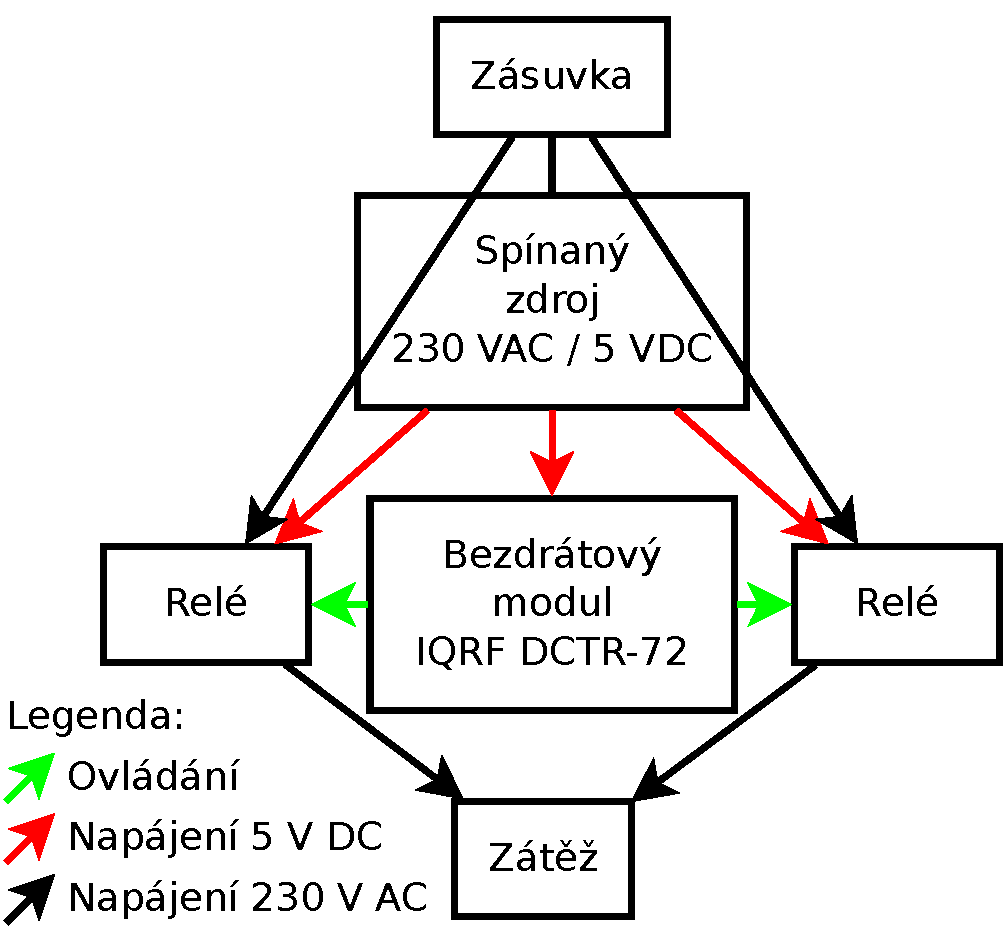
\includegraphics[width = 128mm]{img/blokove-schema-zasuvky.pdf}
\caption{Blokové schéma chytré zásuvky}
\endminipage
\end{figure}

\subsubsection{Obvodové schéma}

\begin{figure}[H]
\label{fig:schematic}
\minipage{\textwidth}
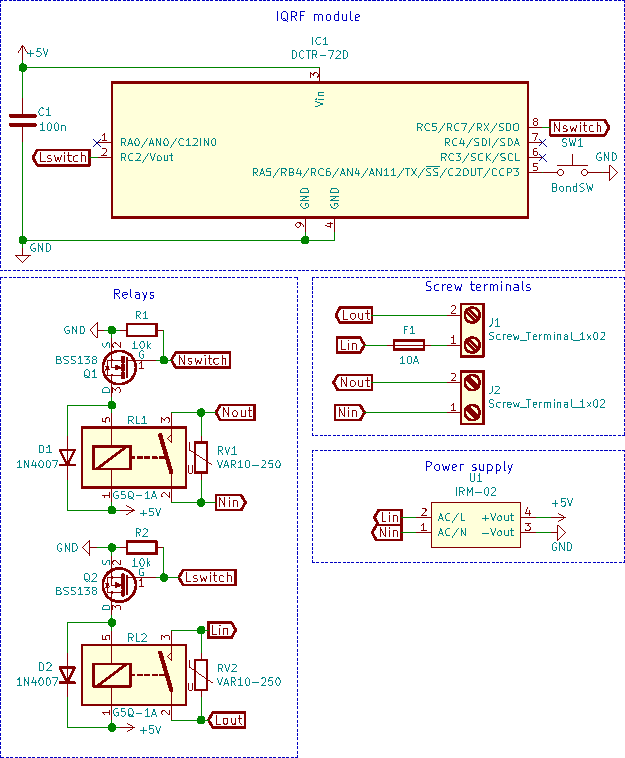
\includegraphics[width = 128mm]{img/schematic.pdf}
\caption{Obvodové schéma chytré zásuvky}
\endminipage
\end{figure}

\subsubsection{Výkres plošného spoje a rozložení součástek}

\begin{figure}[H]
\label{fig:board}
\minipage{\textwidth}
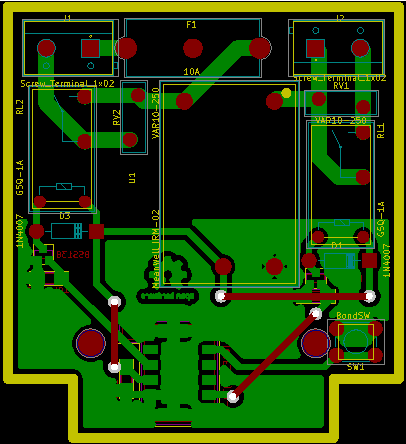
\includegraphics[width = 128mm]{img/board.pdf}
\caption{Výkres plošného spoje chytré zásuvky}
\endminipage
\end{figure}

\begin{figure}[H]
\label{fig:components}
\minipage{\textwidth}
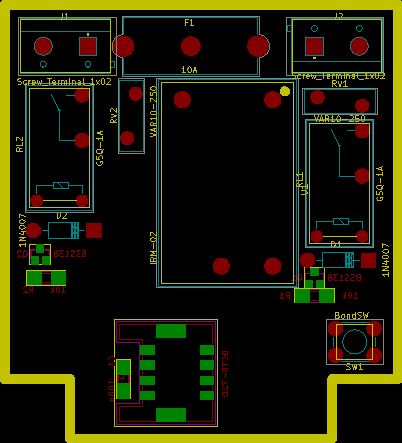
\includegraphics[width = 128mm]{img/components.pdf}
\caption{Rozložení součástek na desce plošného spoje chytré zásuvky}
\endminipage
\end{figure}

\subsubsection{Rozpiska součástek}

\begin{table}[H]
	\centering
	\begin{tabular}{|l|l|}
		\hline 
		\textbf{Značka} & \textbf{Jméno součástky} \\ 
		\hline 
		\hline 
		~ & Krabička COMBIPLAST CP-Z-27/B \\ 
		\hline 
		C1 & Keramický SMD\index[zkr]{SMD!Surface-mounted device|textit} 1206 kondenzátor 100~nF \\ 
		\hline 
		D1, D2 & Dioda 1N4007 \\ 
		\hline 
		F1 & Tavná keramická pojistka 10~A 250~VAC \\ 
		\hline 
		IC1 & Bezdrátový modul IQRF DCTR-72DAT \\ 
		\hline 
		~ & Konektoru IQRF KON-SIM-01 pro IC1 \\ 
		\hline 
		J1, J2 & Svorkovnice do DPS DEGSON DG300-7.5-02P \\ 
		\hline 
		Q1, Q2 & N-MOSFET BSS138 \\ 
		\hline 
		R1, R2 & Rezistor SMD 1206 10~k$\Omega$ \\ 
		\hline 
		RL1, RL2 & Relé OMRON G5Q-1A4-EU 5VDC \\ 
		\hline 
		RV1, RV2 & MOV SR PASSIVES VAR10-250 \\ 
		\hline 
		SW1 & Mikrospínač THT 6$\times$6~mm \\ 
		\hline 
		U1 & Spínaný zdroj MEAN WELL IRM-02-5 \\ 
		\hline 
	\end{tabular}
	\caption{Rozpiska součástek chytré zásuvky}\label{table:rozpiska-soucastek}
\end{table}

\subsection{Brána}

Pro bránu jsem použil linuxový jednodeskový počítač Raspberry Pi 2 model B. Bezdrátový modul IQRF DCTR-72DAT je k bráně připojen přes sběrnici SPI pomocí adaptéru IQRF KON-RASP-01. Pro komunikaci s GSM sítí lze použít USB GSM/3G modem (například Huawei E3131) nebo starší mobilní telefon (například Samsung Star II nebo Samsung Galaxy Gio). Brána se napájí pomocí externího spínaného zdroje s microUSB konektorem, který má výstupní napětí 5~V a maximální výstupní proud 2~A.

\section{Software}

\subsection{Chytrá zásuvka}

Software chytré zásuvky je psán v programovacím jazyce C. 

\subsubsection{IQRF OS}

\subsubsection{IQRF DPA}

\subsection{Brána}

V bráně běží linuxová distribuce Raspbian, což je speciálně upravená linuxová distribuce pro jednodeskový počítač Raspberry Pi. Tato linuxová distribuce je odvozená od linuxové distribuce Debian, která je jedna z nejpoužívanějších linuxových distribucích. Software brány je psán v skriptovacím jazyce Python.

\subsubsection{AT příkazy}

AT příkazy se používají pro komunikaci s GSM modemem. 

\newpage

\section{Technické parametry}

\subsection{Chytrá zásuvka}

\begin{table}[H]
	\centering
	\begin{tabular}{lr}
		\hline 
		\textbf{Technické parametry} & ~ \\ 
		\hline 
		\hline 
		\textbf{Rozměry} & 7$\times$12$\times$4,5~cm \\ 
		\textbf{Hmotnost} & x~g \\ 
		\hline
		\textbf{Elektrické parametry} \\ 
		\hline 
		\hline 
		\textbf{Napájecí napětí} & 90~V až 250~V AC \\ 
		\textbf{Maximální spotřeba} & 400~mA \\ 
		\textbf{Maximální spínatelný proud} &  10~A \\ 
		\hline 
		\textbf{Ostatní parametry} \\ 
		\hline 
		\hline 
		\textbf{Přenos dat} & bezdrátově na frekvenci 868~MHz \\ 
		\textbf{Protokol} & IQRF DPA \\ 
	\end{tabular}
	\caption{Parametry chytré zásuvky}\label{table:parametry/chytra-zasuvka}
\end{table}

\subsection{Brána}

\newpage

\section*{Závěr}

\addcontentsline{toc}{section}{Závěr}

Výsledkem této práce je funkční chytrá zásuvka, která splňuje veškeré požadavky.

\newpage

\printindex[zkr]

\addcontentsline{toc}{section}{Seznam použitých zkratek}

\newpage

\begin{thebibliography}{99}

\addcontentsline{toc}{section}{Seznam použité literatury}

\bibitem{wiki-ism-band}
Wikipedia. ISM Band \emph{Wikipedia} [online]. [cit. 2016-01-08]. \\ Dostupné z: \url{https://en.wikipedia.org/wiki/ISM\_band}

\bibitem{iqrf-os}
MICRORISC. Operating system \emph{IQRF} [online]. Jičín, 2016 [cit. 2017-01-09]. \\ Dostupné z: \url{http://iqrf.org/technology/operating-system}

\bibitem{iqrf-dpa}
MICRORISC. DPA \emph{IQRF} [online]. Jičín, 2016 [cit. 2017-01-09]. \\ Dostupné z: \url{http://iqrf.org/technology/dpa}

\bibitem{iqrf-dctr-72d-datasheet}
MICRORISC. Datasheet DCTR-72D \emph{IQRF} [online]. Jičín, 2016 [cit. 2017-01-09]. \\ Dostupné z: \url{http://iqrf.org/weben/downloads.php?id=337}

\bibitem{robodoupe-mosfet-a-rele}
Jiri Bezstarosti. Tranzistor jako spínač \emph{Robodoupě} [online]. 2012 [cit. 2017-01-09]. \\ Dostupné z: \url{http://robodoupe.cz/2012/tranzistor-jako-spinac/}

\end{thebibliography}

\newpage

\listoffigures

\addcontentsline{toc}{section}{Seznam obrázků}

\listoftables

\addcontentsline{toc}{section}{Seznam tabulek}

\end{document}